\documentclass{beamer}

\usepackage[utf8]{inputenc}
\usepackage{graphicx}
\usepackage{ragged2e}
\usepackage{braket}

\usetheme{Warsaw}

% Macro to add page number

\newcommand*\oldmacro{}%
\let\oldmacro\insertshorttitle%
\renewcommand*\insertshorttitle{%
   \oldmacro\hfill%
   \insertframenumber\,/\,\inserttotalframenumber}

% Graphics information

\graphicspath{{./Figures/}}

% Title page information

\title[Intro MCTDH]{A \emph{gentle} introduction to MCTDH}
\subtitle{\footnotesize With emphasis in potential representations}
\author[Panadés-Barrueta]{Ramón L. Panadés-Barrueta}
\institute{Computational Chemical Physics Group. \\ University of Twente.}
\date{\small November 5, 2020}
\titlegraphic{
\includegraphics[width=1.65cm]{trex_logo.png}\hspace*{7.00cm}~%
   
\includegraphics[width=2cm]{ut_logo.pdf}}

% ToC in each section

\AtBeginSection[]
{
  \begin{frame}
    \tableofcontents[currentsection]
  \end{frame}
}

% Presentation's content

\begin{document}

\frame{\titlepage}

\begin{frame}
  \tableofcontents
\end{frame}

\section{Nuclear Quantum Dynamics}
\label{nqd}

\begin{frame}
  \frametitle{Nuclear Quantum Dynamics}
  \begin{block}{What}
   \justifying
   The subfield of Theoretical Chemistry in which both the \textbf{electrons} and the \textbf{nuclei} of
   a molecular system are treated in a \textbf{quantum-mechanical} manner. 
  \end{block}
  \begin{exampleblock}{When}<2->
    \begin{itemize}
    \item Spectroscopy (e.g. IR transitions)
    \item Quantum tunneling
    \item Strong vibronic coupling
    \item Accurate ZPE determination
    \end{itemize}
  \end{exampleblock}
\end{frame}

\begin{frame}
  \frametitle{Nuclear Quantum Dynamics}
  Find the numerical solution of the TDSE truncating the Hilbert space to a finite dimension (Galerkin's method):
\begin{equation}
  i\hbar\frac{\partial\Psi}{\partial t} = \hat{H}\Psi
\end{equation}
Given a parametric representation of the WF (\(\Psi\)), the optimal solution can be found using the Dirac-Frenkel Variational Principle (DF-VP):
\begin{equation}
	\braket{\delta\Psi|\hat{H}-i\frac{\partial }{\partial t}|\Psi} = 0
\end{equation}
\end{frame}

\subsection{The Standard method}
\label{stdmeth}
\begin{frame}
  \frametitle{The Standard method}
  Simplest representation of the WF:
\begin{equation}
	\Psi(q_i,\ldots, q_f, t) = \sum_{j_1=1}^{N_1}\cdots\sum_{j_f=1}^{N_f} C_{j_1\ldots j_f}(t)\prod_{\kappa=1}^f\varphi^{(\kappa)}_{j_{\kappa}}(q_{\kappa})
	\label{stme}
\end{equation}
After plugging this WF into the DF-VP, and performing the corresponding algebra we obtain
the following EOMs:
\begin{block}{}
\begin{align}
\begin{split}
	i\dot{C}_L &= \sum_J \braket{\varphi_L|\hat{H}|\varphi_J}C_J \\
	\mathbf{C}(t) &= e^{-i\mathbf{H}t}\mathbf{C}(0)
\end{split}
\end{align}
\end{block}
where we have introduced the composite indexes \(J = (j_1,\ldots,j_f)\).

\end{frame}

\subsection{The Time-Dependent Hartree method}
\label{tdh}

\begin{frame}
  \frametitle{A slightly more clever \emph{ansatz}:}
  \justifying{}
  If we now consider time-dependent single-particle functions (SPFs):
\begin{equation}
\Psi(q_1,\ldots, q_f, t) = A(t)\prod^f_{\kappa=1}\varphi_{\kappa}(q_{\kappa}, t)
\end{equation}
and use the DF-VP with arbitrary real constraints \(g_{\kappa} = i\braket{\varphi_{\kappa}(t)|\dot{\varphi}_{\kappa}(t)}\), we get the EOMs:

\begin{block}{}
  \begin{equation}
    \begin{split}
      A(t) &= A(0) \cdot e^{-i\int_0^t E(t')dt'} \\
      i\dot{\varphi}_{\kappa} &= (\mathcal{H}^{(\kappa)} - E)\varphi_{\kappa}
    \end{split}
  \end{equation}
\end{block}
\end{frame}

\begin{frame}
  \frametitle{Main limitations}
  \begin{exampleblock}{Standard method}
    \justifying
    Its application is largely limited due to the \textbf{curse of dimensionality}. Only systems up to four atoms (6D) can be addressed in practice.
  \end{exampleblock}
  \begin{block}{Time-Dependent Hartree}
    A better approach, but physically inaccurate. The \textbf{nuclear correlation} harder to retrieve
    than the electronic correlation. The character of the nuclear WF in inherently \textbf{multiconfigurational}. 
  \end{block}
\end{frame}

\section{The Multiconfiguration Time-Dependent Hartree method}
\label{mctdh}

\begin{frame}
  \frametitle{Ansätze comparison}
  \vspace{-.3cm}
  \begin{block}{Standard Method (CI)}
    \begin{equation}
      \Psi(q_i,\ldots, q_f, t) = \sum_{j_1=1}^{N_1}\cdots\sum_{j_f=1}^{N_f} C_{j_1\ldots j_f}(t)\prod_{\kappa=1}^f\varphi^{(\kappa)}_{j_{\kappa}}(q_{\kappa})
    \end{equation}
  \end{block}
  \begin{exampleblock}{Time-Dependent Hartree (HM)}<2->
    \begin{equation}
      \Psi(q_1,\ldots, q_f, t) = A(t)\prod^f_{\kappa=1}\varphi_{\kappa}(q_{\kappa}, t)
    \end{equation}
  \end{exampleblock}

  \begin{alertblock}{Multiconfiguration Time-Dependent Hartree (MCSCF)}<3->
    \begin{equation}
      \Psi(q_1,\ldots, q_f, t) = \sum^{n_1}_{j_1=1}\cdots\sum^{n_f}_{j_f=1}A_{j_1,\ldots,j_f}(t)\prod^{f}_{\kappa=1}\varphi^{(\kappa)}_{j_{\kappa}}(q_{\kappa}, t)
      \label{mctdh_antz}
    \end{equation}
  \end{alertblock}
\end{frame}

\subsection{EOMs}
\label{eom}

\subsection{Relaxation and block-improved relaxation}
\label{relax}



\section{The problem of the PES}
\label{probpes}
\subsection{Tensor decomposition algorithms}
\label{tdec}

\section{Example application}
\label{applic}
\subsection{The HONO isomerization}
\label{hono}

\subsection[Bibliography]{}
\label{biblio}

\begin{frame}
  \frametitle{Bibliography}
  \centering
  \begin{minipage}{.6\linewidth}
Gatti, F., \emph{et al.} Applications of quantum dynamics in chemistry. Vol. 98.
  Springer, 2017.
\end{minipage}
\hspace{1cm}
  \begin{minipage}{.1\linewidth}
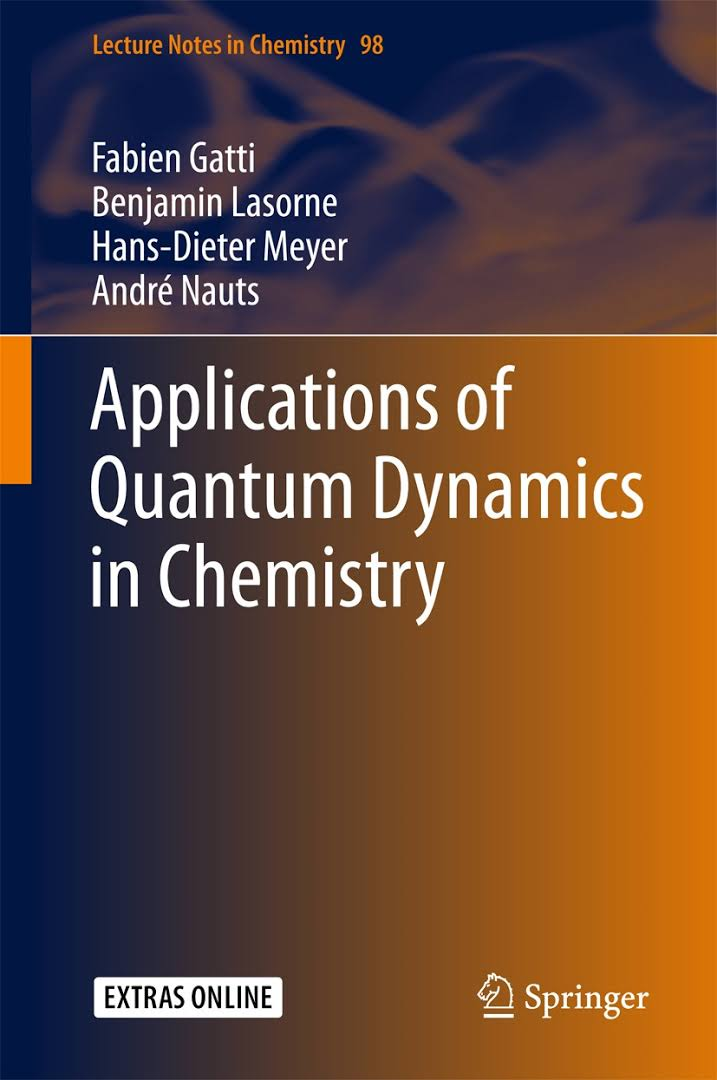
\includegraphics[width=4em]{appli.jpg}
\end{minipage}

\vspace{1cm}

  \begin{minipage}{.6\linewidth}
Beck, M.H., \emph{et al.} The multiconfiguration time-dependent Hartree (MCTDH) method: a highly efficient algorithm for propagating wavepackets. Physics reports 324.1 (2000): 1-105. 
\end{minipage}
\hspace{1cm}
  \begin{minipage}{.1\linewidth}
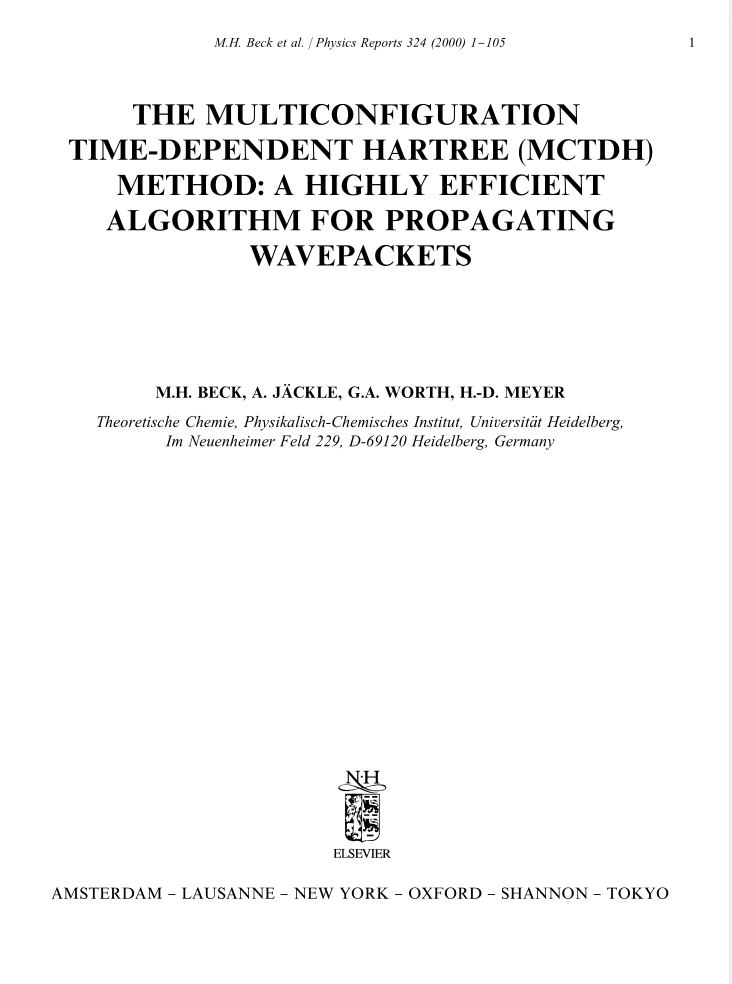
\includegraphics[width=4em]{mctdh_rev.png}
  \end{minipage}
\end{frame}

\begin{frame}
  \centering \Large
  Thanks for your attention!  \\~\\
  Questions?
\end{frame}

\end{document}